\documentclass[twocolumn,3p]{elsarticle}
\usepackage{amsmath}
\usepackage{graphicx}
\usepackage{amssymb}

\begin{document}

\title{High School Assignment}
\author{Adarsh Bhende}

\maketitle

\begin{abstract}
1 ICSE 2019-12th - Problem : 18(a)
\end{abstract}
\section{Problem}
Draw a rough sketch and find the area bounded by curve $x^2=y$ and $x+y=2$
\section {Solution}
The given curve is $x^2=y$ \\
which is an upward parabolawith vertex at origin\\
And line $x+y=2$ i.e,$y=2-x$\\
\begin{align}
x^2&=2-x\\
x^2+x-2&=0\\
(x+2)(x-1)&=0\\
x&=-2 , \\
  x&=1 \\
\end{align}
Now, $y=2-(-2)=4$,\\
$y=2-1=1$\\
Thus,the point of intersection are (-2,4)and(1,1)\\
Required area of shaded region\\
\begin{align}
&=\int\limits_{-2}^{1}(2-x)dx - \int\limits_cx^2dx\\
&=\bigg|2x-\frac{x^2}{2}\bigg|^{1}_{-2}-\bigg|\frac{x^3}{3}\bigg|^{1}_{-2}\\
&=2-\frac{1}{2}+4+\frac{4}{2}-\frac{1}{3}-\frac{8}{3}\\
&=\frac{12-3+24+12-2-16}{6}\\
&=\frac{9}{2}sq.units
\end{align}
\section{Rough Sketch}
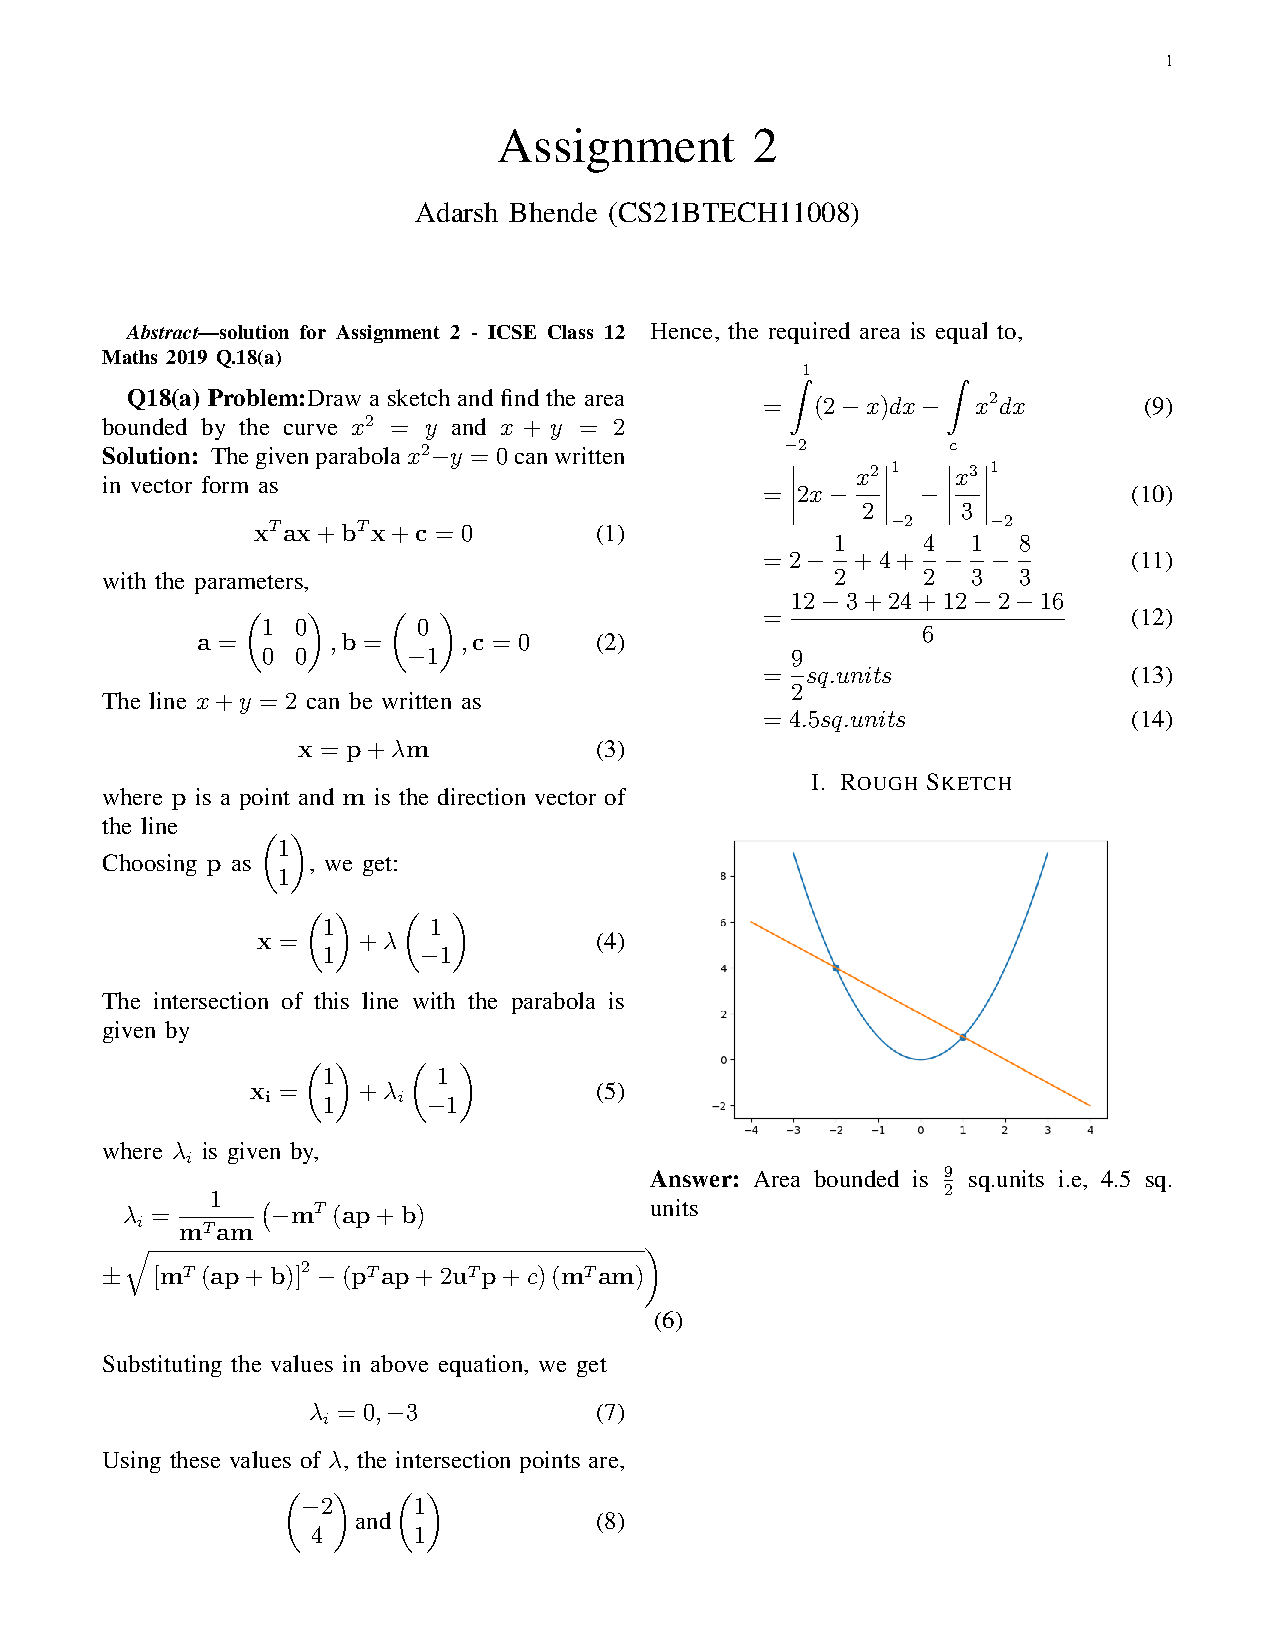
\includegraphics[scale=.5]{main}
\section{Answer}
Area bounded is $\frac{9}{2}$sq.units i.e, 4.5 sq. units\\


\end{document}